\section{Búsqueda}
Holi

\iffalse
% ---- Para poner dos imágenes (una a lado de otra) ----
Como se muestra en la figuras \ref{fig:act-1_a} y \ref{fig:act-1_b}.
\begin{figure}[H]
\centering
\begin{minipage}{0.75\textwidth}
  \centering
  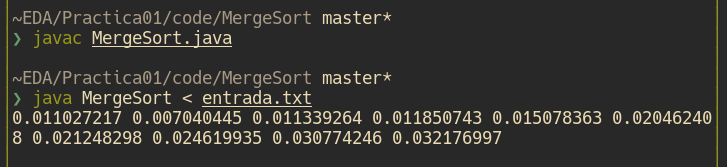
\includegraphics[width=0.8\textwidth]{ejecucion-java}
  \caption{blablablabalbalabla.}
  \label{fig:act-1_a}
\end{minipage}\hfill
\begin{minipage}{0.75\textwidth}
  \centering
  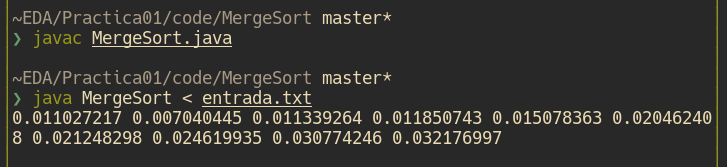
\includegraphics[width=0.8\textwidth]{ejecucion-java}
  \caption{blablablslablala}
  \label{fig:act-1_b}
\end{minipage}
\end{figure}
% ---- Para colocar una imagen ----
Como se muestra en la figura \ref{fig:act-3}
\begin{figure}[H]
  \centering
  \includegraphics[width=0.8\textwidth]{act-3}
  \caption{Tabla de subneteo para la red 192.168.100.0.}
  \label{fig:act-3}
\end{figure}
\fi